% Template last modified by Jake Hart; please contact course staff if you have any questions regarding using this template

\documentclass{cisXXX} % You must have the cisXXX .cls file in your project or working directory (i.e. the same directory as this document) 

\HWauthor{Chen Zhenhao}{20167867} % Put your name and Penn email on this line
\HWno{1} % Enter the number of the homework you are working on
\HWcourse{Compiler} % Enter the course department and number here

%insert a png
%\begin{figure}[ht]
%	\centering
%	
\includegraphics[scale=0.6]{fullscreen.png}
%	\caption{this is a figure demo}
%	\label{fig:label}
%\end{figure}    



\usepackage{graphicx} 
\usepackage{amsmath}
\usepackage{CJK}

\begin{document}
\begin{CJK}{UTF8}{gbsn}
\maketitle


\HWproblem
已知文法 \textbf{G} :
~\\

$<$表达式$>::=<$项$>|<$表达式$>+<$项$>$

$<$项$>::=<$因子$>|<$项$>*<$因子$>$

$<$因子$>::=(<$表达式$>)|$i

~\\
试给出下述表达式的推导及语法树:

\HWsubproblem 
$i$

~\\推导:$<$表达式$>\rightarrow <$项$> \rightarrow <$因子$>\rightarrow i$
%insert a png
\begin{figure}[ht]
	\centering
	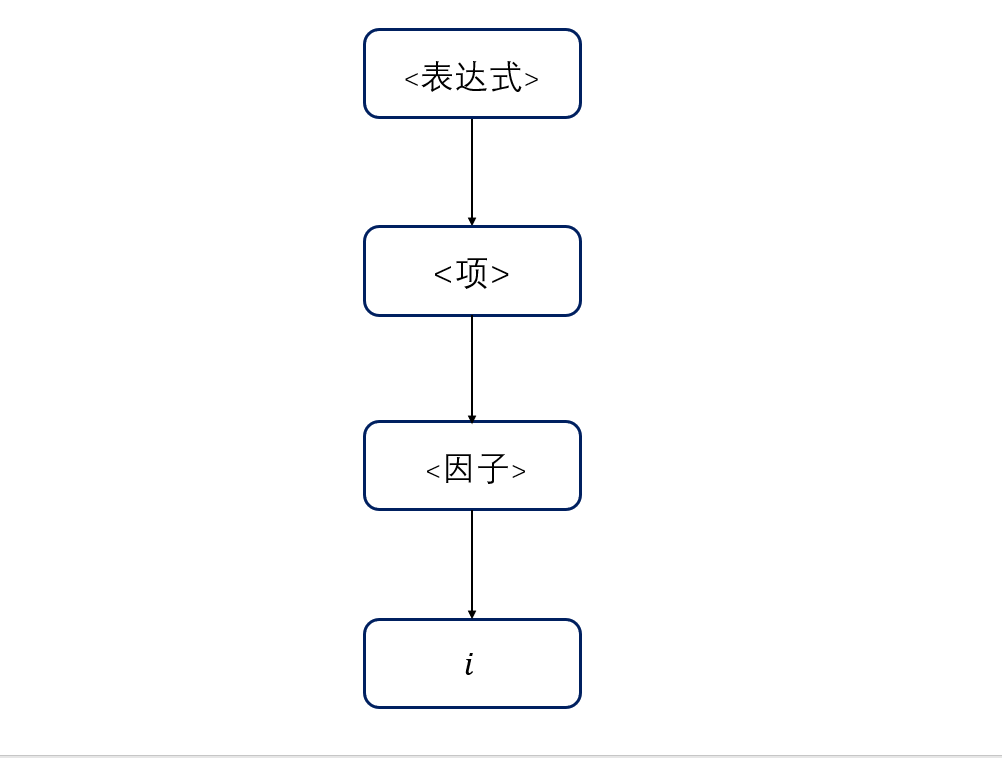
\includegraphics[width=7cm,height=7cm]{1_1.png}
	\caption{$i$的语法树}
	\label{fig:label}
\end{figure}    

\HWsubproblem 
$(i)$

~\\推导:$<$表达式$>\rightarrow <$项$>\rightarrow <$因子$>\rightarrow (<$表达式$>)\rightarrow (<$项$>) \rightarrow (<$因子$>)\rightarrow (i)$
%insert a png
\begin{figure}[ht]
	\centering
	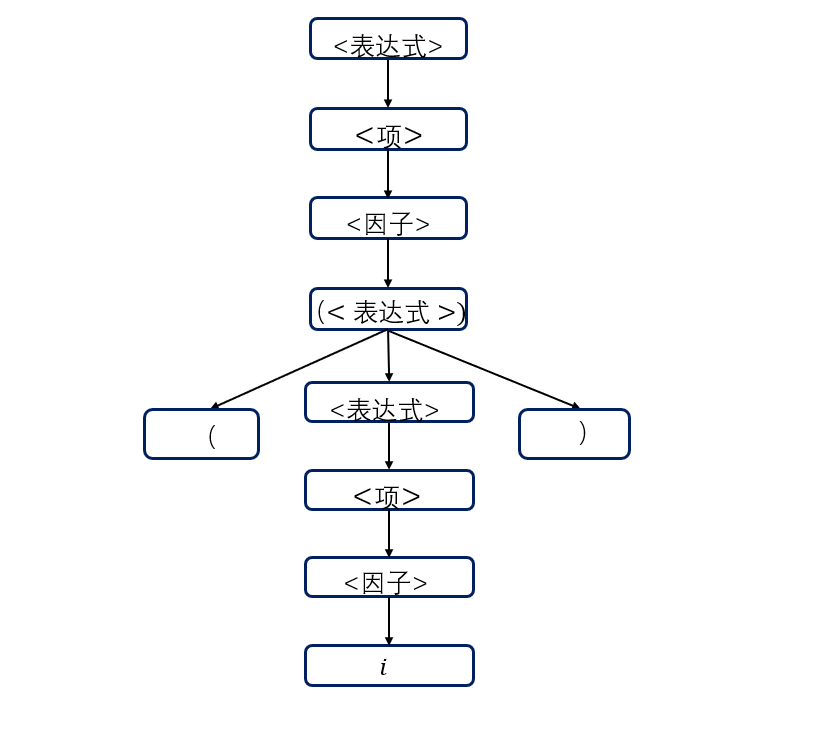
\includegraphics[width=9cm,height=7cm]{1_2.png}
	\caption{$(i)$的语法树}
	\label{fig:label}
\end{figure}    
\HWsubproblem 
$i*i$

~\\推导::$<$表达式$>\rightarrow <$项$>\rightarrow<$项$>*<$因子$>\rightarrow<$项$>*i\rightarrow <$因子$>*i\rightarrow i*i$
\HWsubproblem 
%insert a png
\begin{figure}[ht]
	\centering
	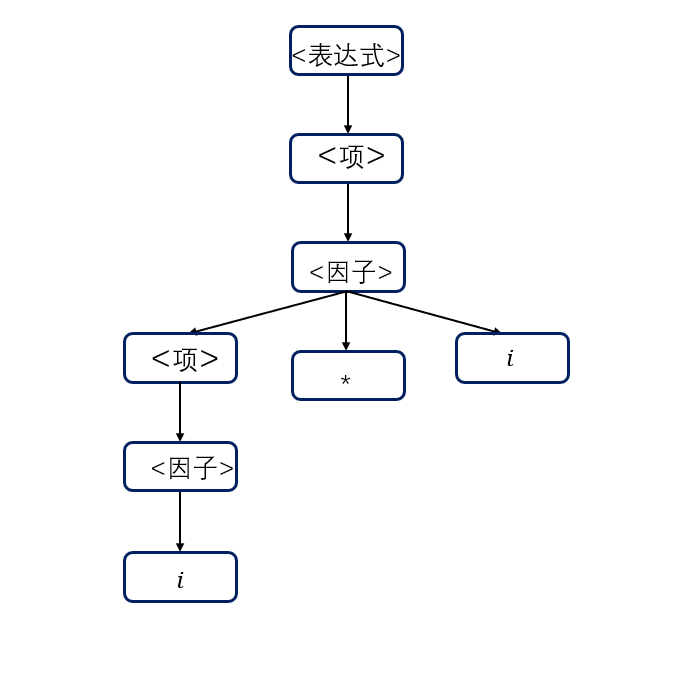
\includegraphics[width=7cm,height=7cm]{1_3.png}
	\caption{$i$的语法树}
	\label{fig:label}
\end{figure}    
$i*i+i$

~\\推导:$<$表达式$>\rightarrow <$表达式$>+<$项$>\rightarrow <$表达式$>+<$因子$>\rightarrow <$表达式$>+i\rightarrow <$项$>+i\rightarrow <$项$>*<$因子$>+i\rightarrow <$项$>*i+i\rightarrow <$因子$>*i+i\rightarrow i*i+i$
%insert a png
\begin{figure}[ht]
	\centering
	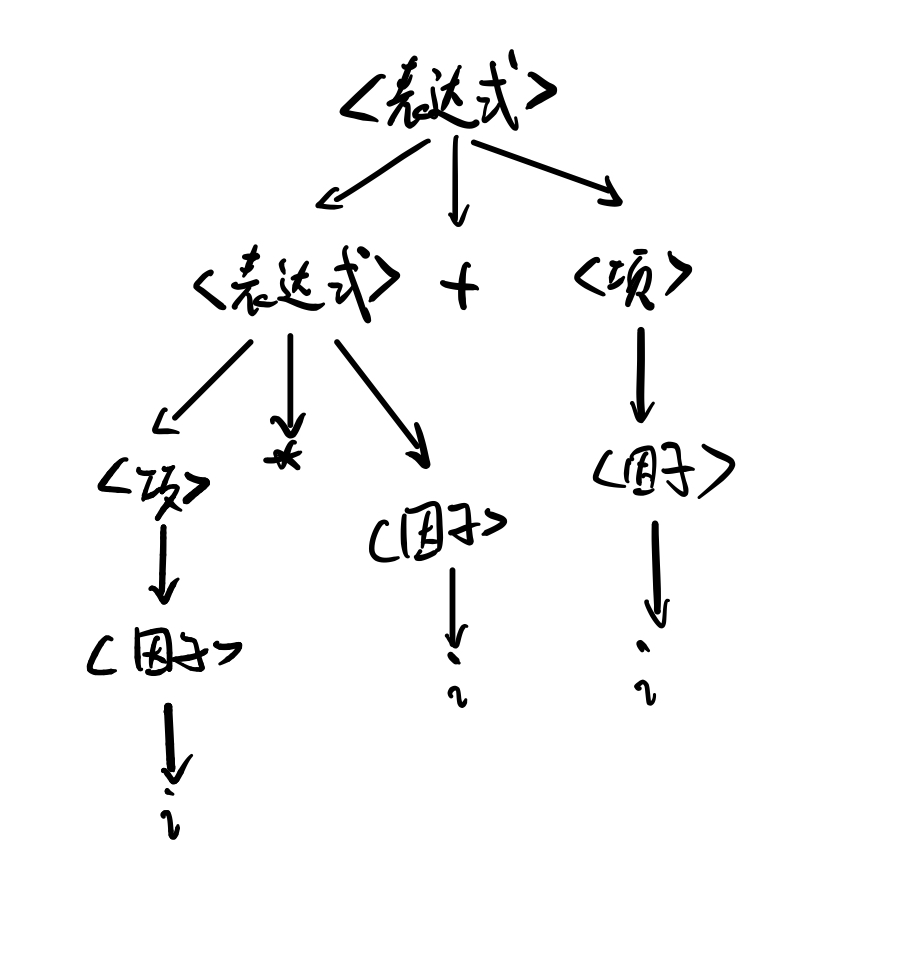
\includegraphics[width=7cm,height=7cm]{1_4.png}
	\caption{$i*i+i$的语法树}
	\label{fig:label}
\end{figure}  
~\\
~\\
~\\
~\\
~\\

\HWsubproblem 


$i+(i+i)$

~\\推导:$<$表达式$>\rightarrow  <$表达式$>+<$项$>\rightarrow  <$表达式$>+ <$因子$>\rightarrow  <$表达式$>+(<$表达式$>)\rightarrow<$表达式$>+(<$表达式$>+<$项$>)\rightarrow<$表达式$>+(<$表达式$>+<$因子$>)\rightarrow<$表达式$>+(<$表达式$>+i)\rightarrow<$表达式$>+(<$项$>+i)\rightarrow<$表达式$>+(<$因子$>+i)\rightarrow<$表达式$>+(i+i)\rightarrow<$项$>+(i+i)\rightarrow<$因子$>+(i+i)\rightarrow i+(i+i)$
%insert a png
\begin{figure}[ht]
	\centering
	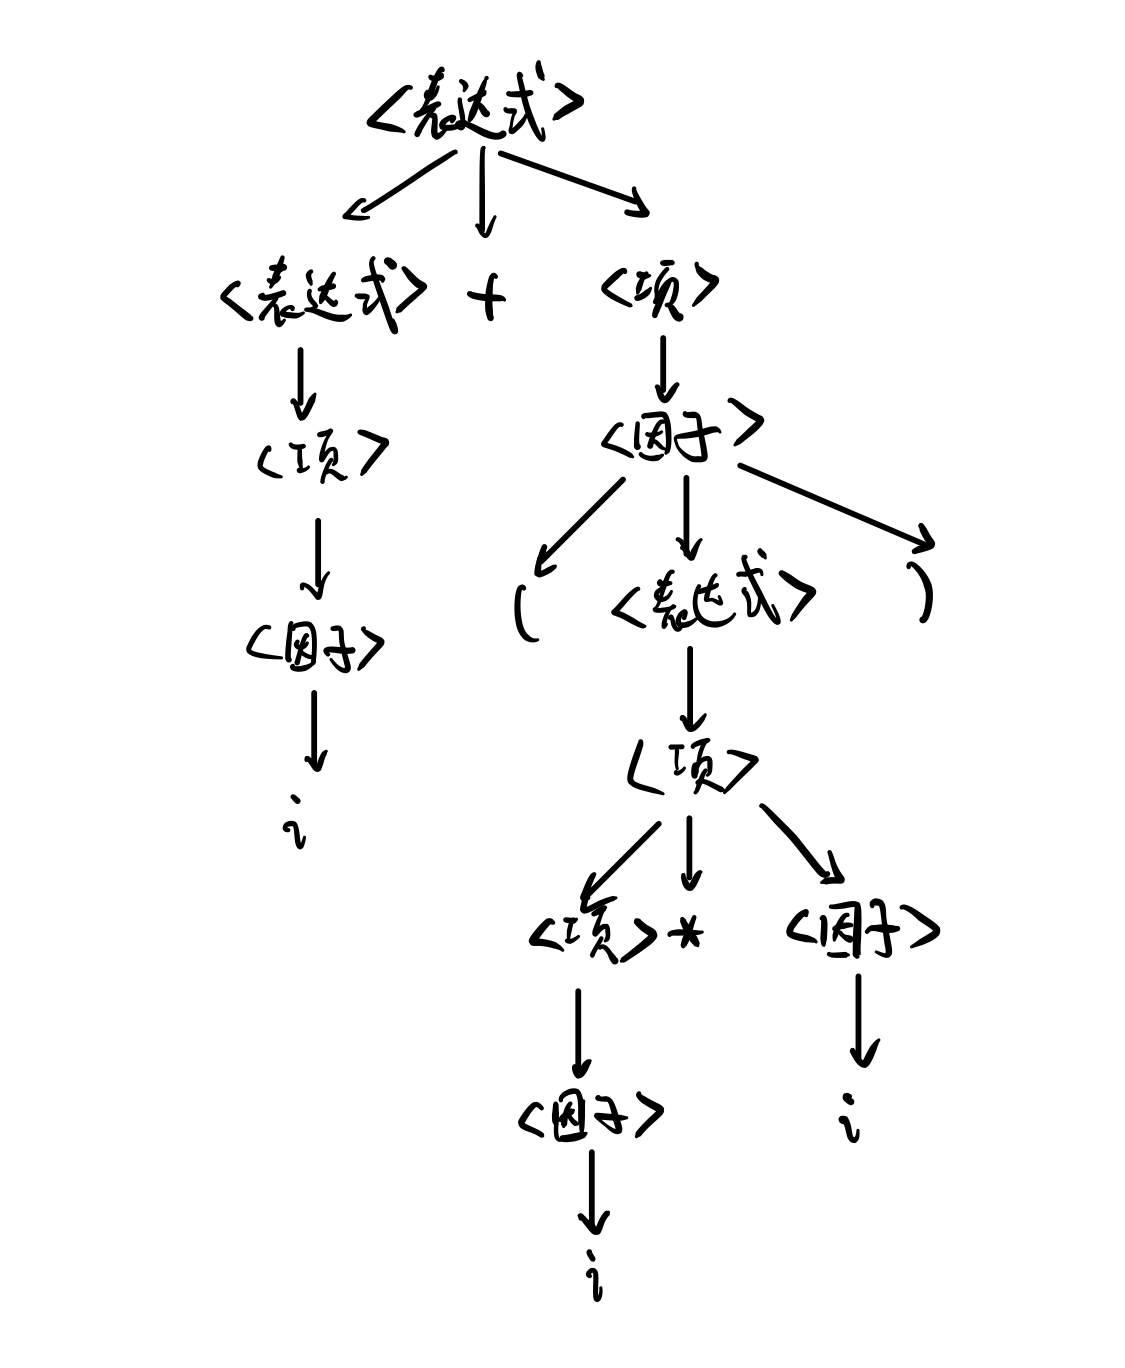
\includegraphics[width=7cm,height=7cm]{1_5.png}
	\caption{$i+(i+i)$的语法树}
	\label{fig:label}
\end{figure}    
\HWsubproblem 
$i+i*i$

~\\推导::$<$表达式$>\rightarrow <$表达式$>+<$项$>\rightarrow <$表达式$>+<$项$>*<$因子$>\rightarrow <$表达式$>+<$项$>*i\rightarrow <$表达式$>+<$因子$>*i\rightarrow <$表达式$>+i*i\rightarrow <$项$>+i*i\rightarrow <$因子$>+i*i\rightarrow i+i*i$
%insert a png
\begin{figure}[ht]
	\centering
	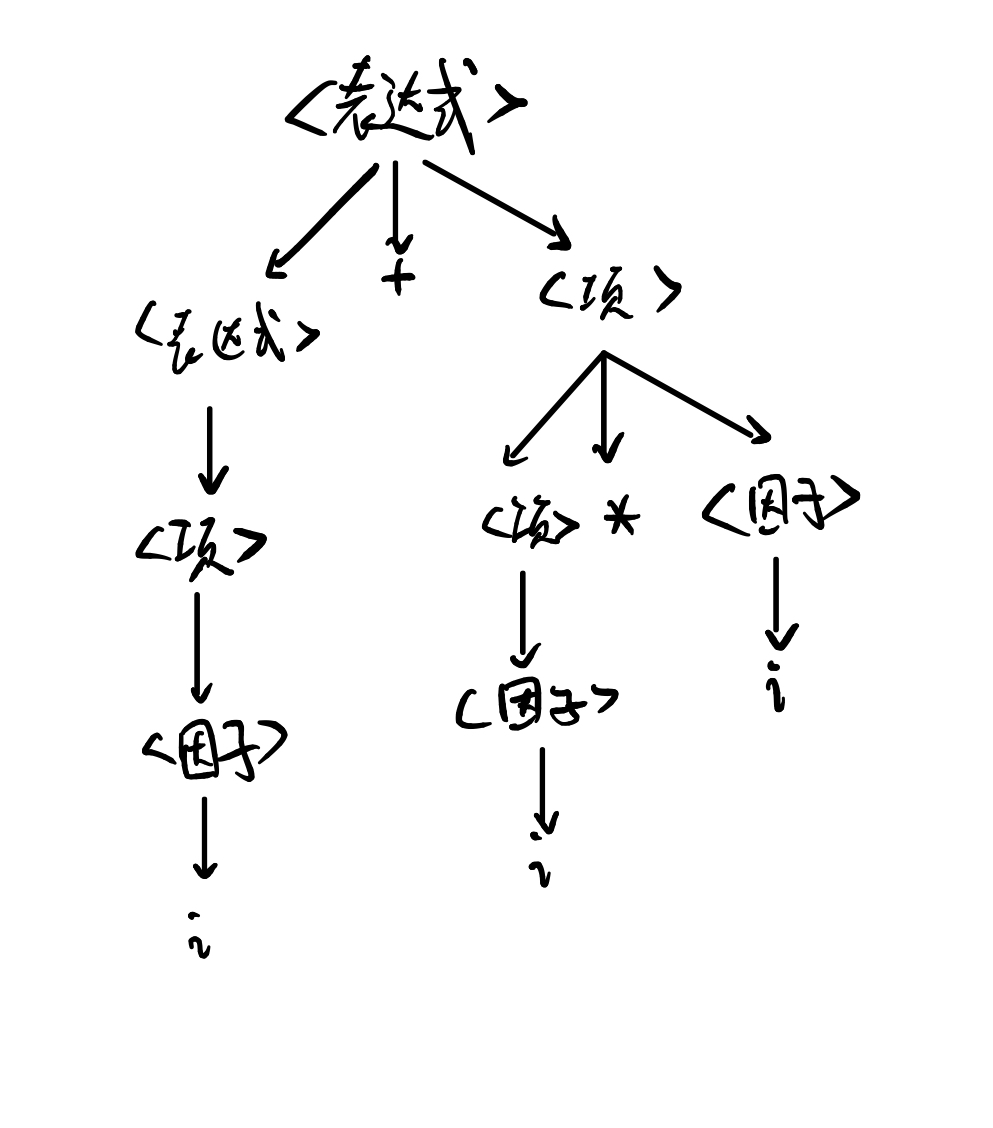
\includegraphics[width=7cm,height=7cm]{1_6.png}
	\caption{$i+i*i$的语法树}
	\label{fig:label}
\end{figure}  
~\\
~\\
~\\
  
\HWproblem
考虑上下文无关文法:\quad $ S \rightarrow SS * | SS+|a $
\HWsubproblem
表明通过此文法如何生成串$aa+a*$,并为该串构造语法树。
~\\

$S\rightarrow SS*\rightarrow Sa*\rightarrow SS+a*\rightarrow Sa+a*\rightarrow aa+a*$

%insert a png
\begin{figure}[ht]
	\centering
	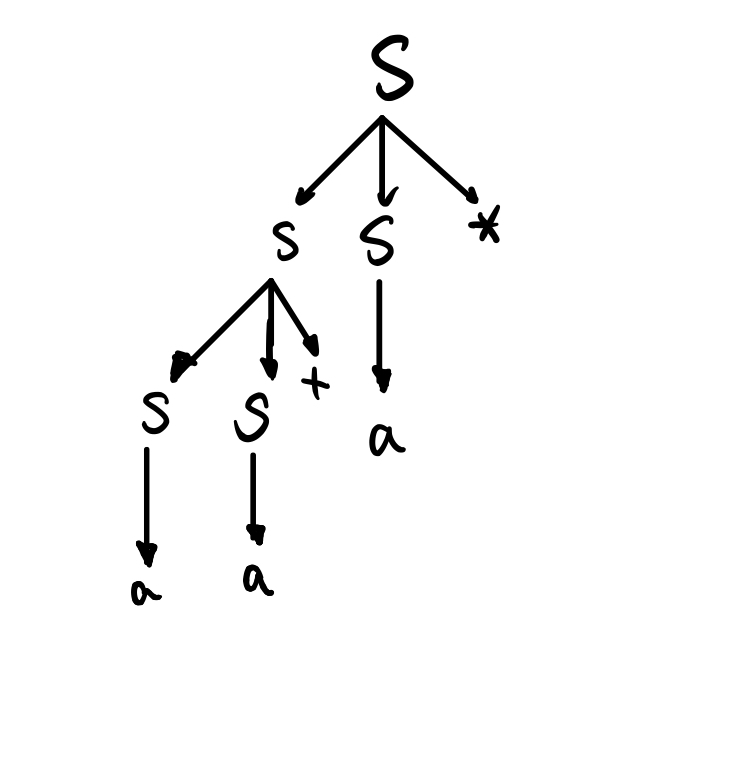
\includegraphics[width=7cm,height=7cm]{2.png}
	\caption{$aa+a*$的语法树}
	\label{fig:label}
\end{figure}    

\HWsubproblem
该文法生成的语言是什么?
~\\

该文法生成的是一个项均为a的且只包含$+$与$-$运算的二则运算式的逆波兰表达式
\HWproblem
已知文法$S\rightarrow S(S)S| \epsilon $。
\HWsubproblem
该文法生成的语言是什么?
~\\

生成了一串括号栈(所有左右括号都满足优先级配对原则)
\HWsubproblem
该文法是二义的吗?说明理由。
~\\

是二义的,如 ()()可以是左右两个不同的\textbf{S} 分别推导得到
\HWproblem
令文法$G[E]$为:

~\\
$E\rightarrow T|E+T|E-T$

~\\
$T\rightarrow F|T*F|T|F$

~\\
$F\rightarrow (E)|i$

~\\
证明:$E+T*F$是它的一个右句型,指出这个句型的所有短语,直接短语和句柄

~\\
证明如下:
~\\

$E\rightarrow E+T\rightarrow E+T*F$

~\\

相对于$E$ 的短语:\quad$E+T*F$

相对于$T$的短语:\quad$T*F$

直接短语:\quad$T*F$

句柄:\quad$T*F$

\HWproblem
一个上下文无关文法生成句子$abbaa$的唯一语法树如下:

%insert a png
\begin{figure}[ht]
	\centering
	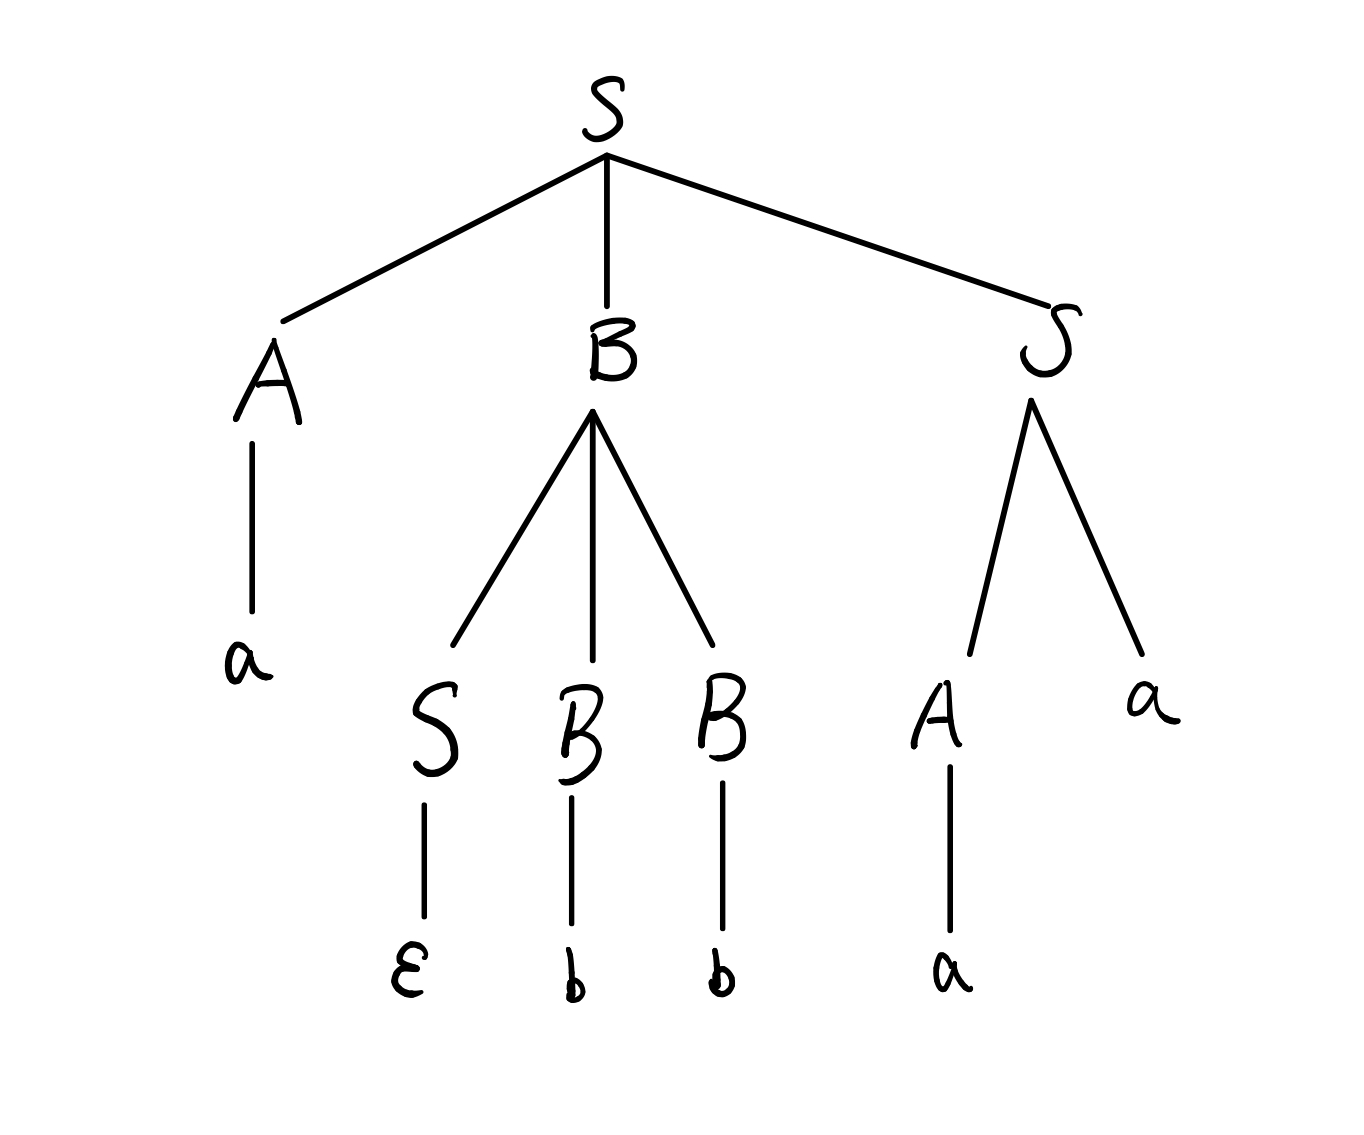
\includegraphics[width=7cm,height=7cm]{5.png}
	\caption{句子$abbaa$的唯一语法树}
	\label{fig:label}
\end{figure}  
~\\
~\\
~\\
~\\
~\\
~\\
~\\
~\\
~\\
\HWsubproblem
给出该句子相应的最左推导与最右推导。

~\\
最左推导:

$S\rightarrow ABS \rightarrow aBS \rightarrow aSBBS \rightarrow abbS \rightarrow abbAa \rightarrow abbaa$

~\\
最右推导:

$S\rightarrow ABS \rightarrow ABAa \rightarrow ABaa \rightarrow ASBBaa \rightarrow Abbaa \rightarrow abbaa$

\HWsubproblem
该文法的产生式集合\textbf{P}可能有哪些元素?

~\\
\textbf{P}中包含了:
~\\

$S\rightarrow ABS|Aa|\epsilon $

$A\rightarrow a$

$B\rightarrow SBB|b$

~\\
\textbf{P}中可能元素有:
~\\

$\epsilon \quad aa \quad ab \quad abbaa \quad ....$\quad.etc

\HWsubproblem
找出该句子的所有短语、简单短语、句柄。

~\\
短语:
~\\

$a$ 是相对 $A$ 的短语
~\\

$\epsilon$是相对$S$的短语
~\\

$b$是相对$B$的短语
~\\

$\epsilon bb$是相对$B$的短语
~\\

$aa$是相对$S$的短语
~\\

$a\epsilon bbaa$是相对$S$的短语

~\\
直接短语:$a \quad \epsilon \quad b$

~\\
句柄:\quad $a$



\HWproblem
给出下述正规文法所对应的正规式:

$S\rightarrow 0A|1B$
~\\

$A\rightarrow 1S|1$
~\\

$B\rightarrow 0S|0$

~\\
将\quad$A\rightarrow 1S|1$\quad 与\quad $B\rightarrow 0S|0$\quad 代入 \textbf{S} 中,得:
~\\

$S\rightarrow0(1S|1)|1(0S|0) \rightarrow (01S|01)|(10S|10) \rightarrow (01|10)S|(01|10) \rightarrow (01|10)^{*}|(01|10)$

~\\
遂正规式为:$(01|10)^{*}|(01|10)$
\end{CJK}
\end{document}
